%!TEX root = ../thesis.tex
%*******************************************************************************
%****************************** Chương 3 ***************************************
%*******************************************************************************

\chapter{DỮ LIỆU VÀ PHƯƠNG PHÁP}
\label{chap:methods}

\ifpdf
    \graphicspath{{Chapter3/Figs/Raster/}{Chapter3/Figs/PDF/}{Chapter3/Figs/}}
\else
    \graphicspath{{Chapter3/Figs/Vector/}{Chapter3/Figs/}}
\fi

\nomenclature[z-ViT]{ViT}{Vision Transformer: bộ mã hóa ảnh dạng transformer, chia ảnh thành các ô (patch)}
\nomenclature[z-MLP]{MLP}{Multi-Layer Perceptron: mạng nơ-ron truyền thẳng nhiều lớp}
\nomenclature[z-bf16]{bf16}{bfloat16: số thực 16 bit có dải giá trị rộng như fp32}
\nomenclature[z-EXIF]{EXIF}{Thông tin kèm file ảnh, gồm cờ cho biết ảnh cần xoay khi hiển thị}
\nomenclature[z-CI95]{CI95}{Khoảng tin cậy 95\%}
\nomenclature[z-ECE]{ECE}{Expected Calibration Error: sai lệch giữa độ tin cậy và độ chính xác thực tế}

Chương này mô tả cách khóa luận trả lời bốn câu hỏi nghiên cứu ở
Chương~\ref{chap:intro}. Mục~\ref{sec:met-overview} tóm tắt quy trình và danh
sách các lần chạy. Mục~\ref{sec:met-data} trình bày hai bộ dữ liệu, cách chia tập
và tiền xử lý. Mục~\ref{sec:met-baseline} mô tả mô hình nền Qwen2.5-VL-3B-Instruct
và việc tái lập nó. Mục~\ref{sec:met-qlora} trình bày cách thích nghi bằng QLoRA,
còn mục~\ref{sec:met-ocr} trình bày cải tiến đề xuất là QLoRA nhận biết OCR.
Mục~\ref{sec:met-eval} nêu giao thức đánh giá, mục~\ref{sec:met-setup} nêu thiết
lập thí nghiệm, và mục~\ref{sec:met-proto} mô tả thiết kế prototype web.

%********************************** Mục 3.1 ************************************
\section{Tổng quan quy trình}
\label{sec:met-overview}

Mọi lần chạy đi qua cùng một quy trình tám bước, chia thành ba giai đoạn:

\begin{description}
  \item[A. Chuẩn bị dữ liệu (chạy một lần, lưu cache).] (1) tải dữ liệu gốc,
  (2) tiền xử lý, (3) OCR các ảnh của ViTextVQA, (4) chia tập cố định.
  \item[B. Huấn luyện và suy luận (giống hệt cho mọi lần chạy).] (5) ghép prompt,
  (6) đưa qua Qwen2.5-VL-3B-Instruct, có hoặc không có adapter LoRA.
  \item[C. Đánh giá và sản phẩm.] (7) chấm điểm và phân tích lỗi, (8) đóng gói
  thành prototype web.
\end{description}

Các phương án được so sánh chỉ khác nhau ở hai ``công tắc'': có đưa dòng chữ OCR
vào prompt hay không (bước 3 và 5), và có huấn luyện adapter LoRA hay không
(bước 6). Mọi yếu tố khác (split, seed, độ phân giải ảnh, kiểu số, cách sinh câu
trả lời, hàm chấm điểm) được giữ cố định, để chênh lệch đo được chỉ do công tắc
gây ra. Hình~\ref{fig:met-pipeline} minh họa quy trình, còn
Bảng~\ref{tab:met-runs} liệt kê các lần chạy được nhắc tới trong khóa luận.

\begin{landscape}
\begin{figure}[p]
\centering
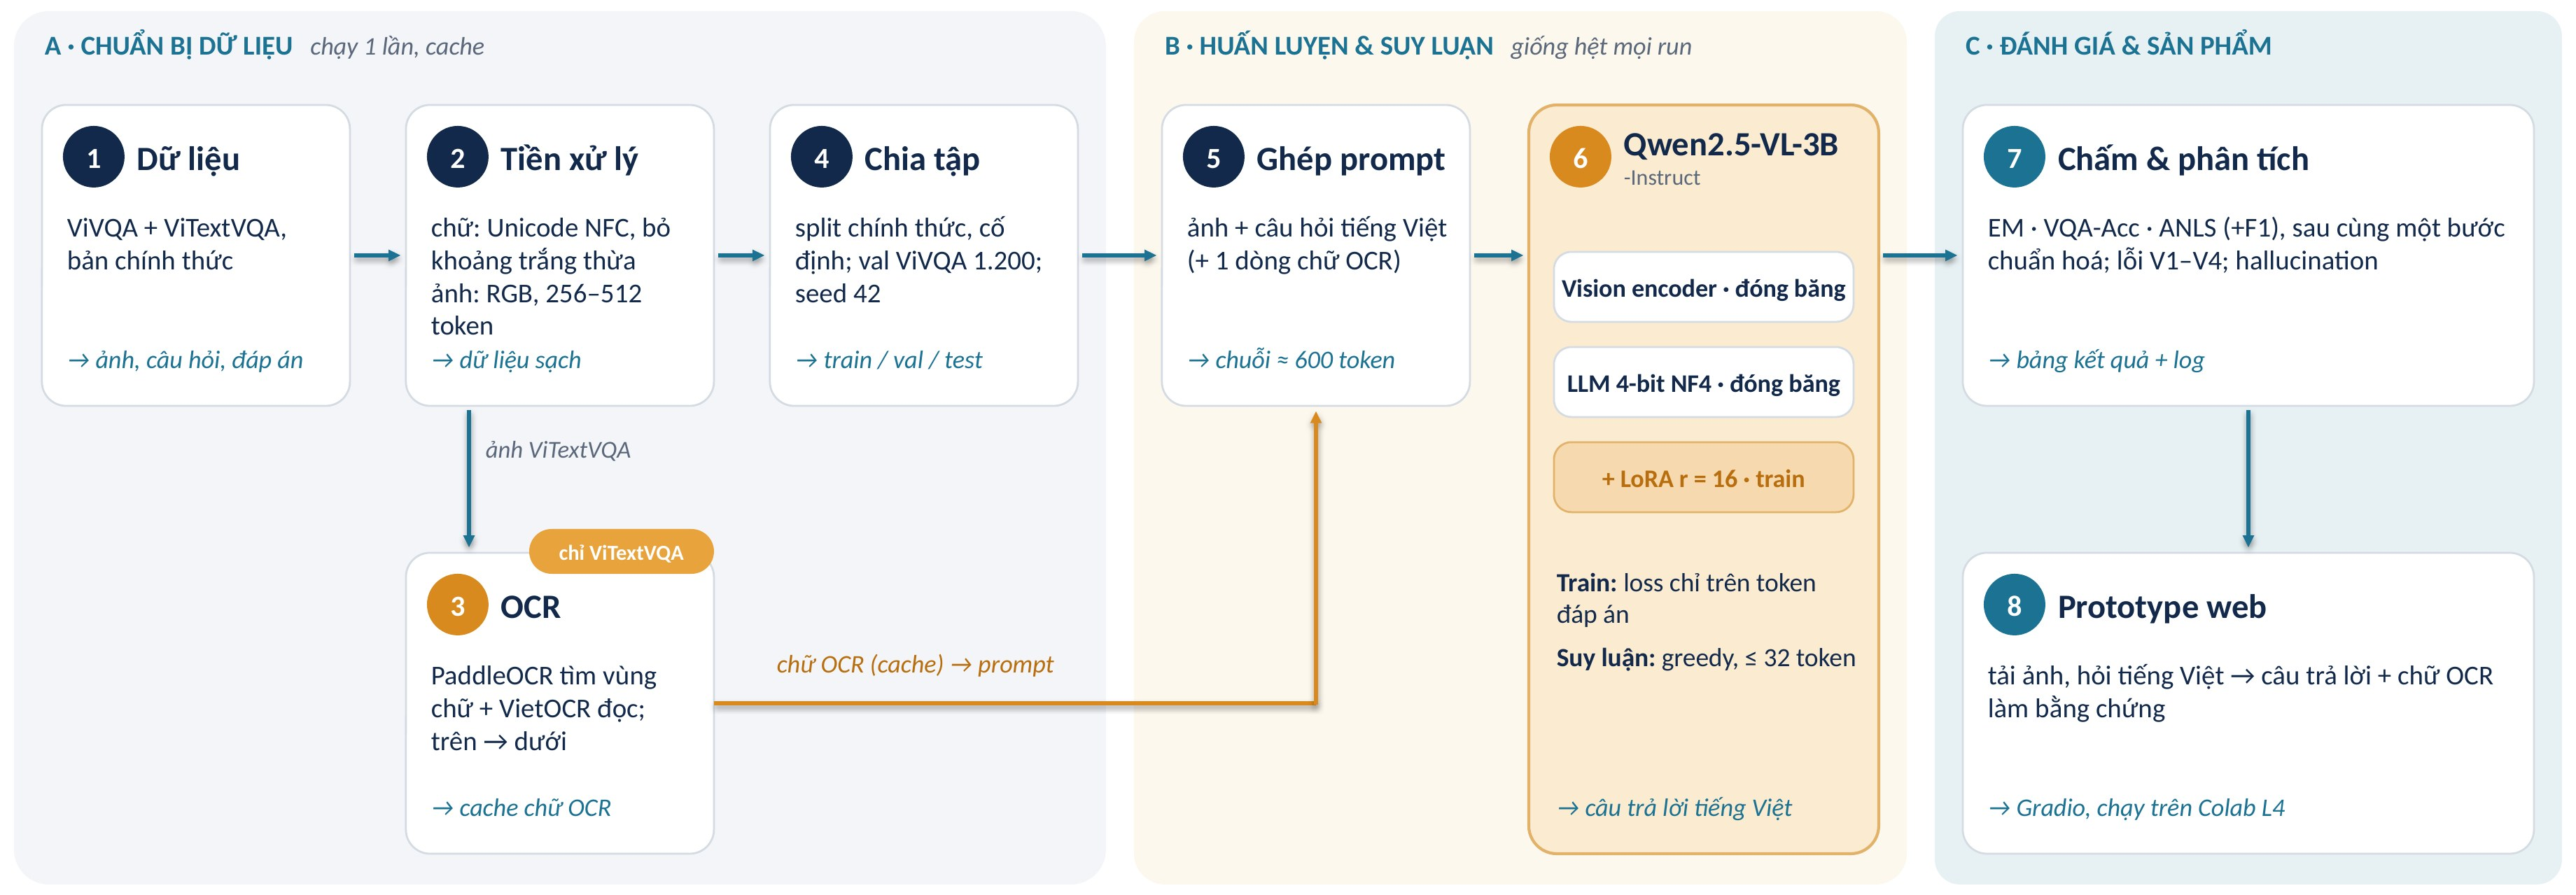
\includegraphics[width=\linewidth,height=0.82\textheight,keepaspectratio]{met_pipeline.jpg}
\caption{Quy trình tám bước. Bước 3 (OCR) chỉ chạy với ViTextVQA; dòng chữ OCR
được lưu cache rồi ghép vào prompt ở bước 5. B1, B2 và B3 đi qua cùng quy trình, chỉ
khác ở bước 3 và bước 6.}
\label{fig:met-pipeline}
\end{figure}
\end{landscape}

\begin{table}[htbp]
\caption{Các lần chạy chính và vai trò của chúng}
\label{tab:met-runs}
\centering
\small
\begin{tabular}{p{0.12\textwidth}p{0.34\textwidth}p{0.44\textwidth}}
\toprule
\raggedright \textbf{Tên} & \raggedright \textbf{Cấu hình} & \raggedright \textbf{Vai trò} \tabularnewline
\midrule
\raggedright R0 & \raggedright Qwen2.5-VL-3B, cấu hình gốc của paper, bf16 & \raggedright Tái lập số đã công bố trên TextVQA val \tabularnewline
\raggedright B1 & \raggedright Zero-shot, 4-bit, không OCR & \raggedright Baseline trên dữ liệu tiếng Việt (RQ1) \tabularnewline
\raggedright B2 & \raggedright QLoRA, toàn bộ train ViTextVQA, không OCR & \raggedright Đo tác dụng của QLoRA (RQ2) \tabularnewline
\raggedright C1 / C3 & \raggedright QLoRA trên ViVQA, 1 / 2 epoch & \raggedright C3 là mô hình chính thức cho ViVQA \tabularnewline
\raggedright B2-sub & \raggedright QLoRA, tập con 8.000 câu ViTextVQA, không OCR & \raggedright Mốc so sánh có kiểm soát cho B3 \tabularnewline
\raggedright B3 & \raggedright Như B2-sub, có dòng OCR khi train và test & \raggedright Kiểm chứng QLoRA nhận biết OCR (RQ3) \tabularnewline
\raggedright B3-full & \raggedright Như B2, có dòng OCR khi train và test & \raggedright Phương pháp đề xuất; mô hình chính thức cho ViTextVQA \tabularnewline
\raggedright A1 / A2 & \raggedright Công thức B3, đổi lớp gắn LoRA / đổi rank & \raggedright Ablation cấu hình LoRA \tabularnewline
\raggedright SH & \raggedright Một adapter cho cả hai bộ dữ liệu & \raggedright Dùng cho prototype \tabularnewline
\bottomrule
\end{tabular}
\end{table}

%********************************** Mục 3.2 ************************************
\section{Dữ liệu}
\label{sec:met-data}

\subsection{Hai bộ dữ liệu}

Bảng~\ref{tab:met-datasets} so sánh hai bộ dữ liệu. Chúng khác nhau ở nguồn ảnh,
cách tạo câu hỏi và dạng đáp án, nên đặt ra hai yêu cầu khác nhau cho mô hình.

\begin{table}[htbp]
\caption{Hai bộ dữ liệu dùng trong khóa luận}
\label{tab:met-datasets}
\centering
\small
\begin{tabular}{p{0.17\textwidth}p{0.37\textwidth}p{0.37\textwidth}}
\toprule
\raggedright & \textbf{ViVQA}~\cite{tran2021vivqa} & \raggedright \textbf{ViTextVQA}~\cite{nguyen2024vitextvqa} \tabularnewline
\midrule
\raggedright Quy mô & \raggedright 15.000 câu hỏi, 10.328 ảnh & \raggedright 50.342 câu hỏi, 16.762 ảnh \tabularnewline
Nguồn ảnh & Chọn ngẫu nhiên từ MS COCO~\cite{lin2014coco}; ảnh đời thường, gần như không có chữ &
Lấy từ Internet và ảnh tự chụp ở Việt Nam; mọi ảnh đều có chữ tiếng Việt \\
Cách tạo câu hỏi & Bán tự động: dịch máy các cặp hỏi--đáp của COCO-QA~\cite{ren2015cocoqa} sang tiếng Việt rồi người kiểm lại &
Gán nhãn tay bởi 16 người bản ngữ; kiểm chéo đạt F1 trên 85\% \\
Loại câu hỏi & 4 loại kế thừa COCO-QA: vật thể, số lượng, màu sắc, vị trí; không có câu có/không &
Hỏi về chữ trong ảnh: tên, địa điểm, sản phẩm, số liên hệ\ldots; không có nhãn loại \\
\raggedright Đáp án & \raggedright Rất ngắn: 99,83\% không quá 3 từ & \raggedright Cụm chữ chép từ ảnh, trung bình 4,18 từ \tabularnewline
\raggedright Thước đo phù hợp & \raggedright EM, VQA-Acc & \raggedright EM, ANLS \tabularnewline
\bottomrule
\end{tabular}
\end{table}

\subsection{Chia tập}
\label{sec:met-split}

\paragraph{ViVQA.} Bản gốc chỉ có hai file \texttt{train.csv} và
\texttt{test.csv}. Nhóm xáo trộn tập train với seed 42 và tách 10\% làm tập val,
được 10.799 câu train và 1.200 câu val; tập test 3.001 câu giữ nguyên. Việc tách
val là quyết định của nhóm, không phải của tác giả bộ dữ liệu.

\paragraph{ViTextVQA.} Nhóm dùng split chính thức của tác giả (tỉ lệ 7:1:2):
35.159 câu train trên 11.733 ảnh, 5.155 câu dev trên 1.676 ảnh và 10.028 câu test
trên 3.353 ảnh. Tập train và tập dev không có ảnh nào trùng với tập test.

\paragraph{Các tập con cố định.} Để thí nghiệm nhanh mà vẫn so sánh được, nhóm
tạo thêm các tập con, mỗi tập chọn một lần bằng seed 42 và lưu danh sách mã câu
hỏi:
\begin{itemize}
  \item \textbf{dev300}: 300 câu dev ViTextVQA, dùng để chọn cấu hình (độ phân
  giải, kiểu số, cấu hình OCR);
  \item \textbf{test2000}: 2.000 câu test ViTextVQA, dùng cho các ablation cần
  nhiều lần chạy;
  \item \textbf{train8k}: 8.000 câu train ViTextVQA trên 2.670 ảnh, dùng cho
  B2-sub, B3 và các ablation;
  \item \textbf{val sạch} ViVQA: 688 câu val có ảnh không xuất hiện trong train,
  dùng để chọn số epoch;
  \item \textbf{test sạch} ViVQA: 1.219 câu test có ảnh không xuất hiện trong
  train, dùng để kiểm tra rò rỉ.
\end{itemize}

Nguyên tắc chung: mọi lựa chọn cấu hình được thực hiện trên dev hoặc val, không
bao giờ trên test. Tập test chỉ dùng để báo cáo.

\subsection{Tiền xử lý: từ file gốc đến bản ghi sạch}
\label{sec:met-prep}

\paragraph{ViVQA.} Script chuẩn bị tải hai file CSV từ kho của tác giả, bỏ cột chỉ
số, giải mã cột loại câu hỏi (0--3 thành vật thể, số lượng, màu sắc, vị trí),
chuẩn hóa câu hỏi và đáp án về Unicode NFC và bỏ khoảng trắng thừa ở hai đầu.
Ảnh được tải từ MS COCO 2014 theo mã ảnh; bản ghi nào có ảnh hỏng bị loại.

\paragraph{ViTextVQA.} Dữ liệu được tải từ kho chính thức trên Hugging Face (cần
đồng ý điều khoản, giấy phép CC BY-NC 3.0). File chú thích dạng COCO (danh sách
ảnh và danh sách chú thích) được làm phẳng thành một dòng cho mỗi câu hỏi. Script
kiểm tra tự động số câu của từng tập, mã câu hỏi không trùng và không có đáp án
rỗng. Kiểm tra này quan trọng vì kho có file \path{ViTextVQA_test.json} là mẫu
nộp bài Kaggle với mọi đáp án là chuỗi giữ chỗ; đáp án thật nằm trong
\path{ViTextVQA_test_gt.json}. Dùng nhầm file mẫu sẽ cho điểm vô nghĩa mà không
báo lỗi. Mã băm SHA-256 của các file gốc được ghi vào báo cáo chuẩn bị để khóa
phiên bản dữ liệu.

\paragraph{Bản ghi chuẩn.} Cả hai bộ dữ liệu được đưa về cùng một dạng bản ghi
gồm \texttt{question\_id}, \texttt{question}, \texttt{answers} (luôn là danh
sách), \texttt{image\_path} và \texttt{question\_type}. Trước khi huấn luyện, mẫu
có đáp án rỗng hoặc thiếu ảnh bị loại. Nhóm không sửa nội dung câu hỏi hay đáp
án, không tăng cường dữ liệu và không thêm dữ liệu huấn luyện từ nguồn ngoài.

Ở bước này văn bản chỉ được chuẩn hóa Unicode NFC và bỏ khoảng trắng thừa. Việc
chuyển chữ thường, bỏ dấu câu và các bước chuẩn hóa khác chỉ áp dụng khi chấm
điểm (mục~\ref{sec:met-norm}), để mô hình học sinh đúng đáp án gốc.

\subsection{Chất lượng dữ liệu}
\label{sec:met-quality}

Trước khi huấn luyện, nhóm đo các vấn đề có sẵn trong dữ liệu gốc. Các vấn đề này
được ghi nhận và báo cáo, không được sửa trong dữ liệu:

\begin{itemize}
  \item \textbf{Đáp án gold sai hoặc nhiễu.} Duyệt tay 200 lỗi của B2 cho thấy
  12,5\% là do gold sai (ViVQA 19\%), phần lớn ở các câu hỏi ViVQA dịch máy khó
  hiểu.
  \item \textbf{Ảnh trùng giữa train và test ở ViVQA.} Khoảng 46\% câu test dùng
  ảnh đã có trong train (49\% nếu tính cả val). Đây là lý do nhóm tạo val sạch
  và test sạch ở mục~\ref{sec:met-split}.
  \item \textbf{ViVQA không có câu có/không.} Không có đáp án ``có'' nào trong
  tập train, nên mô hình chỉ học trên ViVQA có nguy cơ quên cách trả lời câu
  có/không (kiểm ở Chương~\ref{chap:discussion}).
  \item \textbf{Gold ViTextVQA viết tách dấu câu}, ví dụ ``0983 . 651 888''
  (25,7\% đáp án). Hàm chuẩn hóa khi chấm xử lý điều này đối xứng cho cả đáp án
  và câu trả lời.
  \item \textbf{Ảnh có cờ xoay EXIF.} Một số ít ảnh ViTextVQA có cờ xoay; ảnh
  hưởng của chúng lên OCR được phân tích ở mục~\ref{sec:res-exif}.
  \item \textbf{ViTextVQA không có nhãn loại câu hỏi.} Nhóm xây một bộ phân loại
  theo luật từ khóa gồm 9 loại (gọi là \texttt{qt-v1}), viết chỉ từ dev300 và
  đóng băng trước khi chạy trên test; kiểm trên 150 câu gán nhãn mù đạt độ chính
  xác 80,7\%.
\end{itemize}

%********************************** Mục 3.3 ************************************
\section{Mô hình nền Qwen2.5-VL-3B-Instruct}
\label{sec:met-baseline}

\subsection{Lý do chọn}

Đề cương cho phép chọn một trong ba baseline BLIP-2, Florence-2 và Qwen2.5-VL.
Nhóm chọn Qwen2.5-VL-3B-Instruct~\cite{bai2025qwen25vl} vì bốn lý do: mô hình hỗ
trợ đa ngôn ngữ, trong đó có tiếng Việt; khả năng đọc chữ trong ảnh tốt (TextVQA
val 79,3 theo báo cáo gốc); kích thước 3 tỉ tham số đủ nhỏ để lượng tử hóa 4-bit
và huấn luyện trên một GPU Colab; và mô hình sinh câu trả lời tự do, phù hợp với
đáp án dạng cụm từ của ViTextVQA. Các VLM khác chỉ được dùng làm tham chiếu
zero-shot.

\subsection{Kiến trúc}

Qwen2.5-VL-3B-Instruct gồm ba khối:

\begin{enumerate}
  \item \textbf{Vision encoder} dạng ViT~\cite{dosovitskiy2021vit} với 32 lớp,
  độ rộng 1.280. Ảnh được cắt thành các ô 14$\times$14 điểm ảnh. Phần lớn các lớp
  dùng window attention, mỗi ô chỉ tính attention trong cửa sổ 112$\times$112
  điểm ảnh để giảm chi phí; bốn lớp (thứ 7, 15, 23, 31) dùng full attention trên
  toàn ảnh.
  \item \textbf{MLP merger} gộp 2$\times$2 ô kề nhau thành một token và chiếu
  sang không gian 2.048 chiều của mô hình ngôn ngữ. Mỗi token ảnh vì vậy ứng với
  một vùng 28$\times$28 điểm ảnh.
  \item \textbf{Mô hình ngôn ngữ Qwen2.5} gồm 36 lớp decoder, độ rộng 2.048,
  dùng grouped-query attention với 16 đầu query và 2 đầu key--value, mỗi đầu 128
  chiều. Mô hình đọc chuỗi token ảnh cùng token chữ và sinh câu trả lời từng
  token một.
\end{enumerate}

Hình~\ref{fig:met-arch} cho thấy đường đi của dữ liệu qua ba khối này, cùng vị trí
gắn adapter LoRA (mục~\ref{sec:met-qlora}).

\begin{landscape}
\begin{figure}[p]
\centering
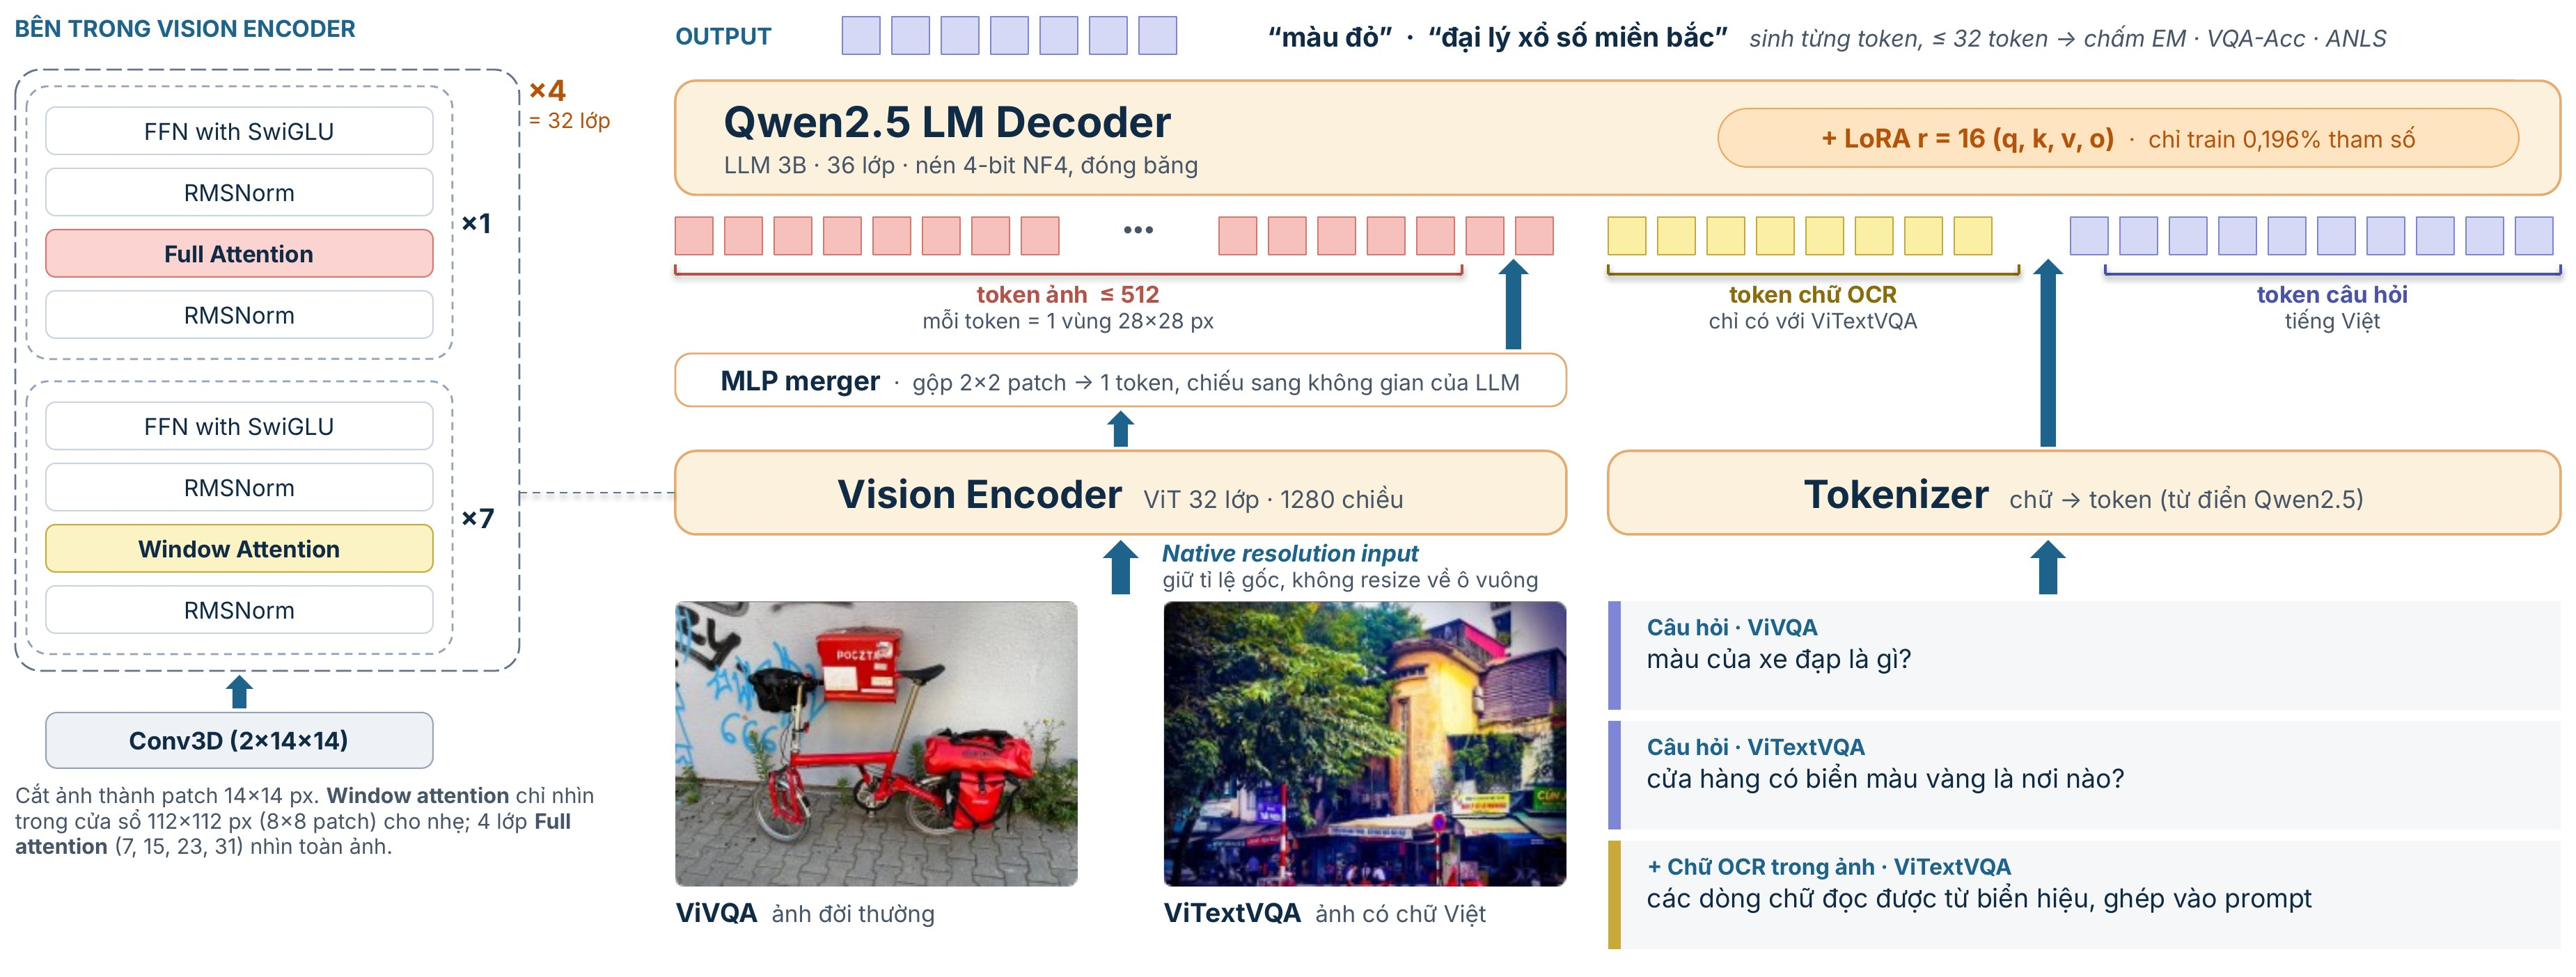
\includegraphics[width=\linewidth,height=0.82\textheight,keepaspectratio]{met_architecture.jpg}
\caption{Qwen2.5-VL-3B-Instruct trong khóa luận: ảnh đi qua Conv3D, vision encoder
và MLP merger thành token ảnh; câu hỏi và chữ OCR đi qua tokenizer thành token chữ;
LM decoder (4-bit, đóng băng, gắn LoRA) đọc cả chuỗi và sinh câu trả lời. Khung bên
trái là cấu trúc một khối của vision encoder. Sơ đồ vẽ lại, phỏng theo Hình 1
trong báo cáo kỹ thuật của Bai và cộng sự~\cite{bai2025qwen25vl}.}
\label{fig:met-arch}
\end{figure}
\end{landscape}

\subsection{Tiền xử lý ảnh}
\label{sec:met-image}

Ảnh được mở và đổi sang RGB, rồi được bộ xử lý ảnh của Qwen2.5-VL đổi kích thước
giữ nguyên tỉ lệ (native resolution): mỗi cạnh làm tròn về bội số của 28 và tổng
số điểm ảnh được ép vào khoảng $[200.704;\ 401.408]$, tức 256 đến 512 token ảnh.
Ảnh lớn bị thu nhỏ, ảnh nhỏ được phóng lên. Sau đó giá trị điểm ảnh được chuẩn
hóa theo trung bình và độ lệch chuẩn của bộ mã hóa ảnh. Hai ví dụ:

\begin{itemize}
  \item Ảnh ViVQA 640$\times$360 điểm ảnh nằm trong khoảng cho phép, chỉ được làm
  tròn cạnh thành 644$\times$364, tức lưới 23$\times$13 = 299 token ảnh.
  \item Ảnh ViTextVQA 1.024$\times$996 điểm ảnh vượt trần, được thu nhỏ còn
  616$\times$616, tức lưới 22$\times$22 = 484 token ảnh.
\end{itemize}

Trên tập test, ảnh ViVQA có trung vị 345 token (tối đa 506; chỉ 1,5\% ảnh chạm
trần), còn ảnh ViTextVQA có trung vị 480 token và 57,7\% ảnh chạm trần 512.
Hình~\ref{fig:met-image} minh họa các bước và hai ví dụ trên.

\begin{landscape}
\begin{figure}[p]
\centering
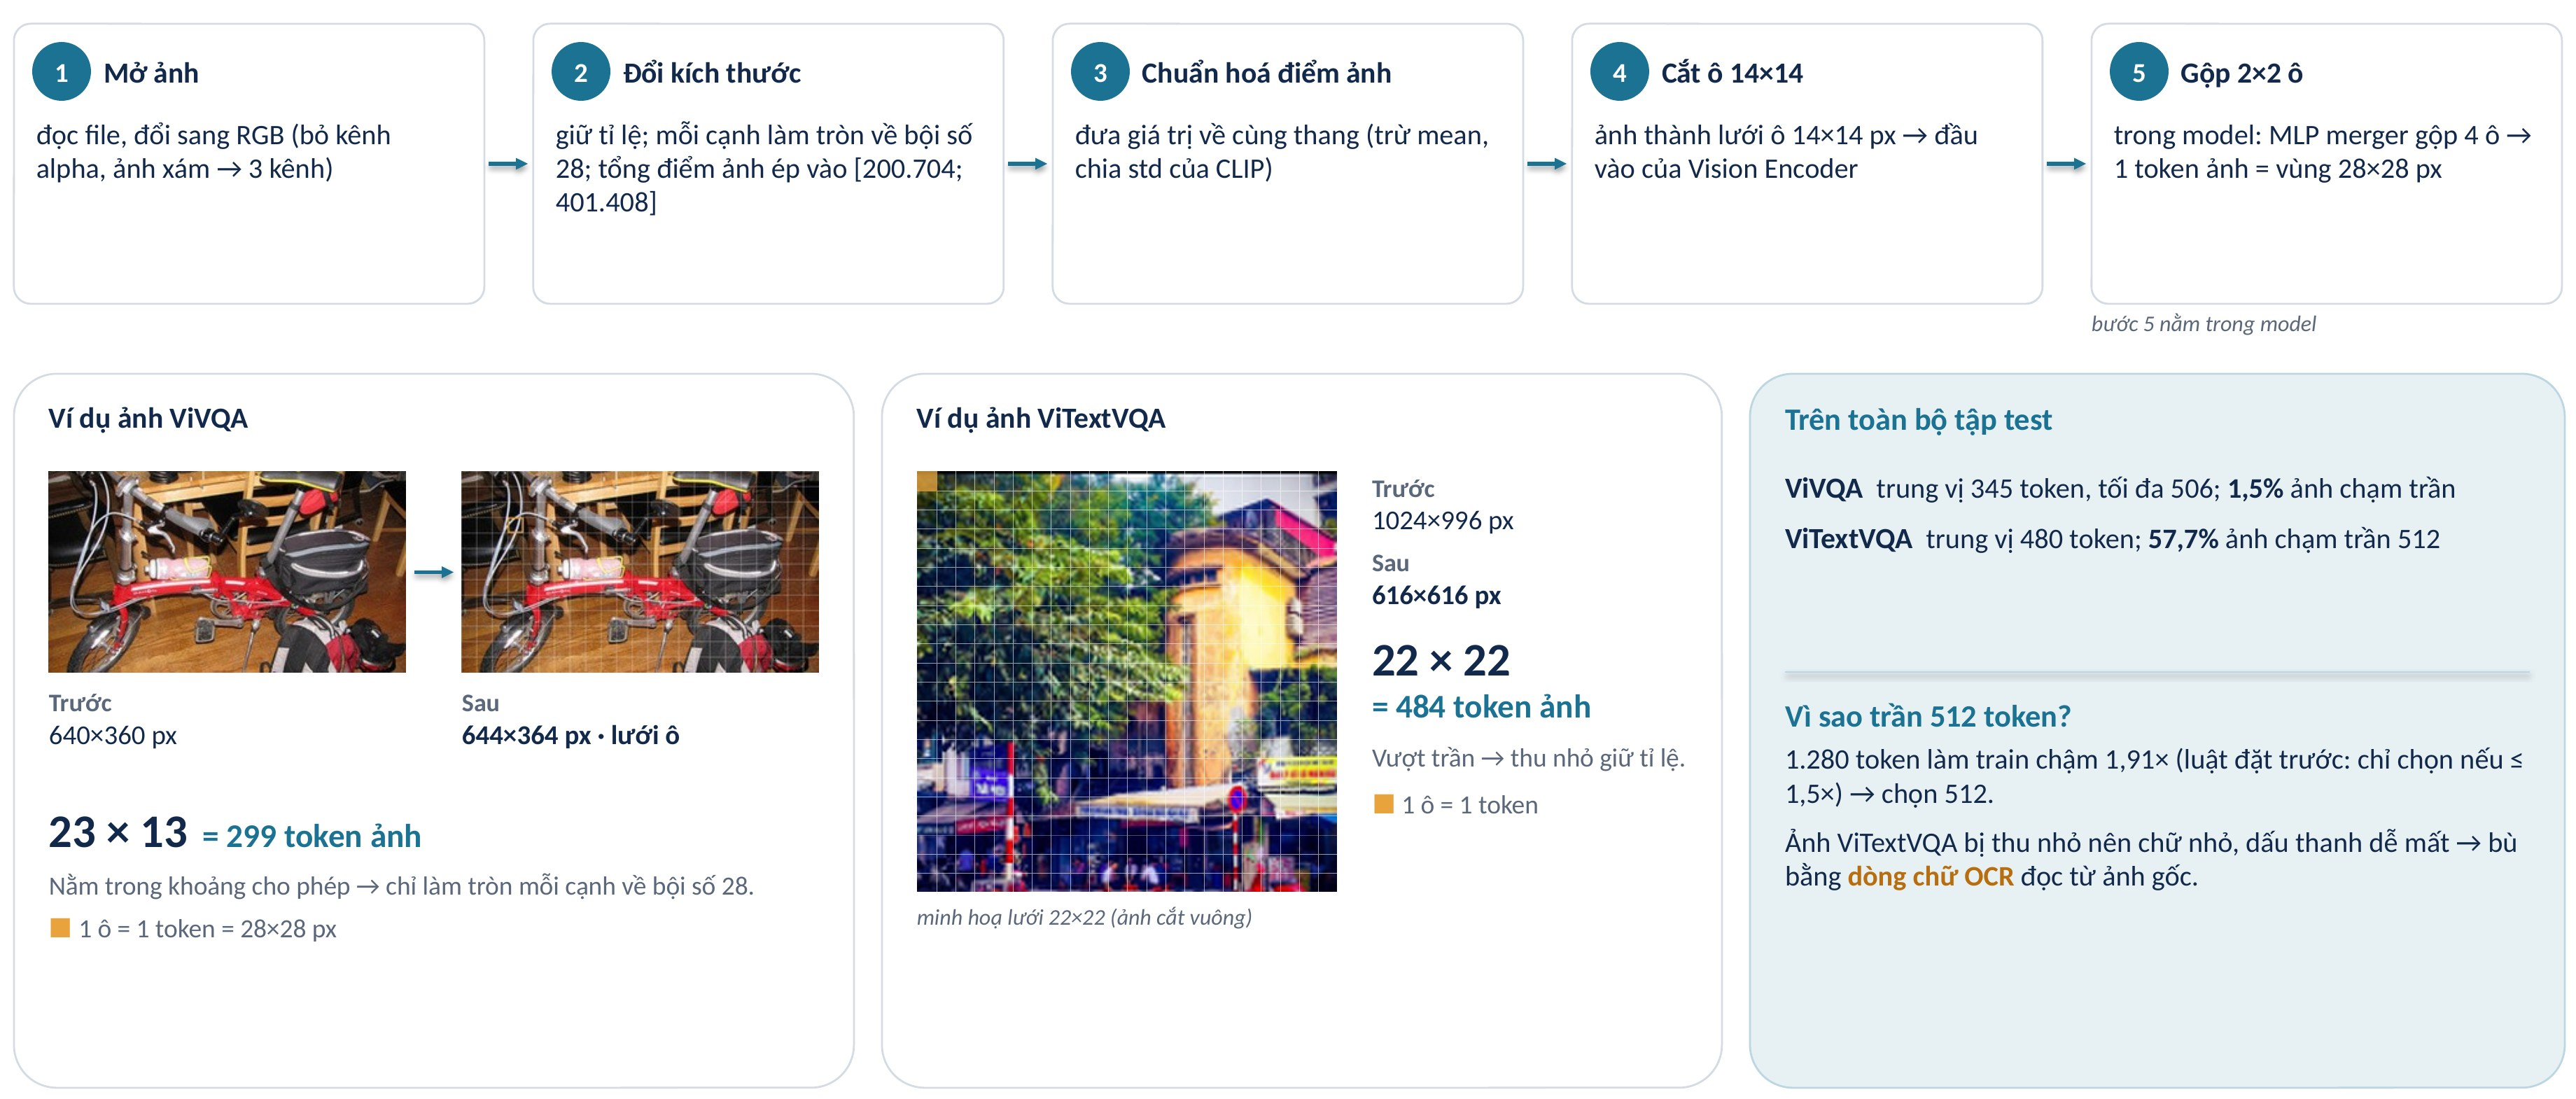
\includegraphics[width=\linewidth,height=0.82\textheight,keepaspectratio]{met_image_tokens.jpg}
\caption{Tiền xử lý ảnh: từ file ảnh đến lưới token ảnh, với một ví dụ ViVQA (chỉ
làm tròn cạnh) và một ví dụ ViTextVQA (thu nhỏ vì vượt trần 512 token). Lưới trên
ảnh ViTextVQA chỉ để minh họa.}
\label{fig:met-image}
\end{figure}
\end{landscape}

\paragraph{Vì sao trần 512 token.} Nhóm đặt luật trước khi đo: chọn 1.280 token
nếu thời gian huấn luyện tăng không quá 1,5 lần. Bảng~\ref{tab:met-res} cho thấy
1.280 token làm thời gian huấn luyện một epoch ViTextVQA tăng 1,91 lần, nên nhóm
chọn 512 token. Phần độ phân giải bị mất, quan trọng với dấu thanh nhỏ trong chữ
tiếng Việt, được bù bằng dòng chữ OCR đọc từ ảnh gốc (mục~\ref{sec:met-ocr}).

\begin{table}[htbp]
\caption{So sánh 512 và 1.280 token ảnh trên ViTextVQA}
\label{tab:met-res}
\centering
\small
\begin{tabular}{p{0.36\textwidth}rrp{0.24\textwidth}}
\toprule
\textbf{Đo} & \textbf{512} & \textbf{1.280} & \textbf{Chênh} \\
\midrule
EM zero-shot (dev300) & 33,3 & 36,0 & +2,7; $p = 0{,}13$ \\
ANLS zero-shot (dev300) & 46,5 & 50,4 & +3,9 [+1,2; +6,6] \\
Thời gian train 1 epoch (L4, giờ) & 11,1 & 21,2 & $\times$1,91 \\
VRAM khi train (GB) & 6,71 & 10,84 & +62\% \\
Suy luận (giây/câu) & 2,61 & 3,81 & $\times$1,46 \\
\bottomrule
\end{tabular}
\end{table}

\subsection{Kiểu số và lượng tử hóa}
\label{sec:met-dtype}

Baseline ban đầu chạy fp16 trên GPU T4 và sinh ra 23 câu trả lời suy biến (chuỗi
dấu ``!'' dài đúng 32 token). Nhóm chẩn đoán đây là tràn số: fp16 chỉ biểu diễn
tới 65.504, logit thành vô cực và phép chọn giá trị lớn nhất rơi về token số 0,
chính là ``!''. Thí nghiệm một biến trên 73 câu (23 câu hỏng và 50 câu đối chứng)
xác nhận: fp16 hỏng 23/73 câu, fp32 và bf16 không hỏng câu nào, trong đó fp32
chậm hơn bf16 1,71 lần. Vì GPU L4 hỗ trợ bf16 còn T4 thì không, mọi lần chạy
chính thức dùng bf16 trên L4.

Trọng số mô hình nền được lượng tử hóa 4-bit NF4 với double
quantization~\cite{dettmers2023qlora}. Mức này giảm VRAM khi suy luận từ 10,9~GB
xuống 2,5~GB và giữ 94,5\% độ chính xác trên TextVQA val
(mục~\ref{sec:res-repro}).

\subsection{Tái lập baseline}

Paper của Qwen2.5-VL không báo cáo trên ViVQA hay ViTextVQA. Vì vậy nhóm tái lập
theo hai bước. Bước một (R0) chạy mô hình với cấu hình gốc của paper trên toàn bộ
5.000 câu TextVQA val, nơi có số công bố, để kiểm tra đường suy luận của nhóm là
đúng. Bước hai (B1) chạy cùng mô hình ở chế độ zero-shot với cấu hình tiết kiệm
của nhóm (4-bit, tối đa 512 token ảnh) trên ViVQA và ViTextVQA, để tạo con số
tham chiếu cho mọi cải tiến. Kết quả cả hai bước nằm ở mục~\ref{sec:res-repro}.

%********************************** Mục 3.4 ************************************
\section{Thích nghi bằng QLoRA}
\label{sec:met-qlora}

\subsection{Cấu hình adapter}

Theo LoRA~\cite{hu2022lora} (phương trình~\ref{eq:lora}), mỗi lớp tuyến tính được
chọn nhận thêm hai ma trận hạng thấp $BA$; chỉ $A$ và $B$ được huấn luyện. Nhóm
gắn adapter vào bốn phép chiếu attention \texttt{q\_proj}, \texttt{k\_proj},
\texttt{v\_proj}, \texttt{o\_proj} của 36 lớp decoder, với rank $r = 16$,
$\alpha = 32$ và dropout 0,05. Mô hình nền được lượng tử hóa 4-bit NF4 và đóng
băng hoàn toàn. Bảng~\ref{tab:met-params} kiểm tra lại số tham số huấn luyện bằng
tính tay.

\begin{table}[htbp]
\caption{Số tham số LoRA theo từng phép chiếu ($r = 16$)}
\label{tab:met-params}
\centering
\small
\begin{tabular}{lcr}
\toprule
\textbf{Phép chiếu} & \textbf{Kích thước (vào $\to$ ra)} & \textbf{Tham số $= r(d_{in}+d_{out})$} \\
\midrule
\texttt{q\_proj} & 2.048 $\to$ 2.048 & 65.536 \\
\texttt{k\_proj} & 2.048 $\to$ 256 & 36.864 \\
\texttt{v\_proj} & 2.048 $\to$ 256 & 36.864 \\
\texttt{o\_proj} & 2.048 $\to$ 2.048 & 65.536 \\
\midrule
Mỗi lớp decoder & & 204.800 \\
$\times$ 36 lớp & & \textbf{7.372.800} \\
\bottomrule
\end{tabular}
\end{table}

Tổng 7.372.800 tham số bằng 0,196\% trong 3,76 tỉ tham số của mô hình, khớp với
số do thư viện PEFT báo cáo. Kết quả khớp cũng cho thấy adapter chỉ nằm trong mô
hình ngôn ngữ: vision encoder và MLP merger không bị chạm tới. Nhóm kiểm thêm
bằng danh sách lớp được gắn LoRA ghi trong log huấn luyện. Adapter lưu ra file
29,5~MB.

\subsection{Nhãn huấn luyện và che nhãn}
\label{sec:met-labels}

Mỗi mẫu huấn luyện là một chuỗi theo khuôn hội thoại của Qwen: câu lệnh hệ thống
cố định, ảnh, phần chữ của prompt (mục~\ref{sec:met-prompt}), rồi đáp án. Câu
lệnh hệ thống là: ``Bạn là trợ lý hỏi đáp hình ảnh tiếng Việt. Hãy trả lời thật
NGẮN GỌN và CHÍNH XÁC bằng tiếng Việt, chỉ đưa ra đáp án, không giải thích dài
dòng.'' Nhãn là đáp án đầu tiên trong danh sách gold, gộp khoảng trắng, giữ nguyên
chữ và dấu, nối thêm token kết thúc lượt \texttt{<|im\_end|>} để mô hình học khi
nào dừng.

Mọi token của câu lệnh hệ thống, ảnh và câu hỏi mang nhãn $-100$ nên bị bỏ qua
khi tính loss. Gọi $\mathcal{A}$ là tập vị trí các token đáp án, hàm mất mát là
\begin{equation}
\mathcal{L} = -\frac{1}{|\mathcal{A}|}\sum_{t \in \mathcal{A}} \log p_\theta\left(y_t \mid y_{<t},\, I,\, x\right),
\label{eq:loss}
\end{equation}
trong đó $I$ là ảnh, $x$ là phần chữ của prompt và $\theta$ chỉ gồm tham số LoRA.
Nếu không che, phần lớn tín hiệu học sẽ dồn vào việc sinh lại hơn 500 token ảnh và
câu hỏi, trong khi đáp án chỉ có vài token. Vì số token ảnh thay đổi theo kích
thước ảnh, độ dài prompt được đo riêng cho từng mẫu bằng cách cho bộ xử lý chạy
trên đúng phần prompt và đúng ảnh đó; chuỗi được đệm bên phải để prompt luôn nằm
đầu chuỗi.

Một hàm dựng prompt duy nhất được dùng cho cả huấn luyện và đánh giá. Nhờ vậy
prompt lúc huấn luyện trùng khít prompt lúc đánh giá, tránh lệch phân phối giữa
hai giai đoạn.

\subsection{Siêu tham số}

Bảng~\ref{tab:met-hparams} liệt kê siêu tham số dùng chung cho mọi lần huấn luyện.
Riêng mô hình chính thức cho ViVQA (C3) dùng lịch hai epoch và lấy adapter sau
epoch thứ hai; số epoch được chọn trên val sạch (mục~\ref{sec:res-qlora}).

\begin{table}[htbp]
\caption{Siêu tham số huấn luyện}
\label{tab:met-hparams}
\centering
\small
\begin{tabular}{p{0.30\textwidth}p{0.58\textwidth}}
\toprule
\textbf{Tham số} & \textbf{Giá trị} \\
\midrule
LoRA & $r = 16$, $\alpha = 32$, dropout 0,05, gắn q, k, v, o của LLM \\
Lượng tử hóa & 4-bit NF4, double quantization, tính toán bf16 \\
Learning rate & $2\times10^{-4}$, warmup 3\% số bước, weight decay 0 \\
Batch & 2 mẫu $\times$ tích lũy gradient 8 = batch hiệu dụng 16 \\
Gradient checkpointing & Bật \\
Số epoch & 1 (C3: 2, chọn trên val sạch) \\
Ảnh & 256--512 token (min\_pixels 200.704, max\_pixels 401.408) \\
Suy luận & Greedy, tối đa 32 token sinh \\
Seed & 42 (kiểm độ ổn định với 42, 43, 44) \\
\bottomrule
\end{tabular}
\end{table}

%********************************** Mục 3.5 ************************************
\section{Phương pháp đề xuất: QLoRA nhận biết OCR}
\label{sec:met-ocr}

\subsection{Động lực}

Duyệt tay 200 lỗi của B2 cho thấy lỗi thật trên ViTextVQA chủ yếu là lỗi đọc
chữ: đọc sai chữ chiếm 28\%, nhầm vùng chữ 23\% và sai dấu thanh 8\% số lỗi. Đây
đúng là hai vấn đề V1 (dấu thanh) và V3 (thứ tự chữ) ở Chương~\ref{chap:intro}.
Ở 512 token ảnh, ảnh ViTextVQA bị thu nhỏ nên các nét dấu nhỏ dễ mất. Một hệ OCR
đọc ảnh ở độ phân giải gốc có thể cung cấp lại thông tin này dưới dạng chữ.

Tuy nhiên, thêm OCR vào prompt của một mô hình chưa từng thấy OCR là không đủ.
Trên dev300, việc thêm dòng OCR khi suy luận làm đổi 167/300 câu trả lời của B1,
nhưng chỉ sửa đúng 16 câu và làm hỏng 16 câu: mô hình dùng OCR không phân biệt.
Từ đó nhóm đề xuất đưa dòng OCR vào prompt \emph{ngay trong lúc huấn luyện}
QLoRA, để adapter học khi nào nên tin và chép từ OCR, khi nào nên bỏ qua. Nhóm
gọi phương pháp này là QLoRA nhận biết OCR (OCR-aware QLoRA).

\subsection{Đường OCR}
\label{sec:met-ocrpipe}

OCR chạy một lần trên ảnh gốc; kết quả được lưu vào cache và mọi lần huấn luyện,
đánh giá chỉ tra cache. Nhờ vậy mọi phương án có OCR dùng đúng cùng một chữ OCR.
Đường OCR gồm sáu bước:

\begin{enumerate}
  \item \textbf{Sửa hướng ảnh} theo cờ EXIF trước khi đọc (bổ sung sau khi phát
  hiện lỗi, mục~\ref{sec:res-exif}).
  \item \textbf{Dò vùng chữ} bằng mô hình dò của PaddleOCR~\cite{du2020ppocr}.
  \item \textbf{Đọc chữ} từng vùng bằng VietOCR~\cite{vietocr} (kiến trúc
  VGG--transformer), mô hình được huấn luyện cho chữ tiếng Việt có dấu.
  \item \textbf{Sắp thứ tự đọc}: các hộp có tâm theo chiều dọc lệch nhau ít hơn
  một nửa chiều cao trung vị được gom vào cùng một dòng; các dòng xếp từ trên
  xuống, trong mỗi dòng xếp từ trái sang phải. Tác giả ViTextVQA đã chỉ ra thứ tự
  trái-trên đến phải-dưới là có ích~\cite{nguyen2024vitextvqa}.
  \item \textbf{Lưu cache}: với mỗi ảnh lưu chữ, độ tin cậy và tọa độ hộp của
  từng dòng; cache được khóa bằng mã băm SHA-256. Lưu cả tọa độ cho phép phân
  tích lỗi ``nhầm vùng chữ'' mà không phải OCR lại.
  \item \textbf{Tạo dòng OCR}: các dòng được nối bằng dấu ``\textbar'', cắt ở 600
  ký tự và thêm tiền tố ``Văn bản đọc được trong ảnh:''.
\end{enumerate}

Cache phủ 15.352 ảnh ViTextVQA (toàn bộ train, test và dev300). Ảnh không đọc ra
chữ nào thì không có dòng OCR, và prompt trùng hệt prompt không OCR.
Hình~\ref{fig:met-ocr} minh họa sáu bước trên một ảnh thật.

\begin{landscape}
\begin{figure}[p]
\centering
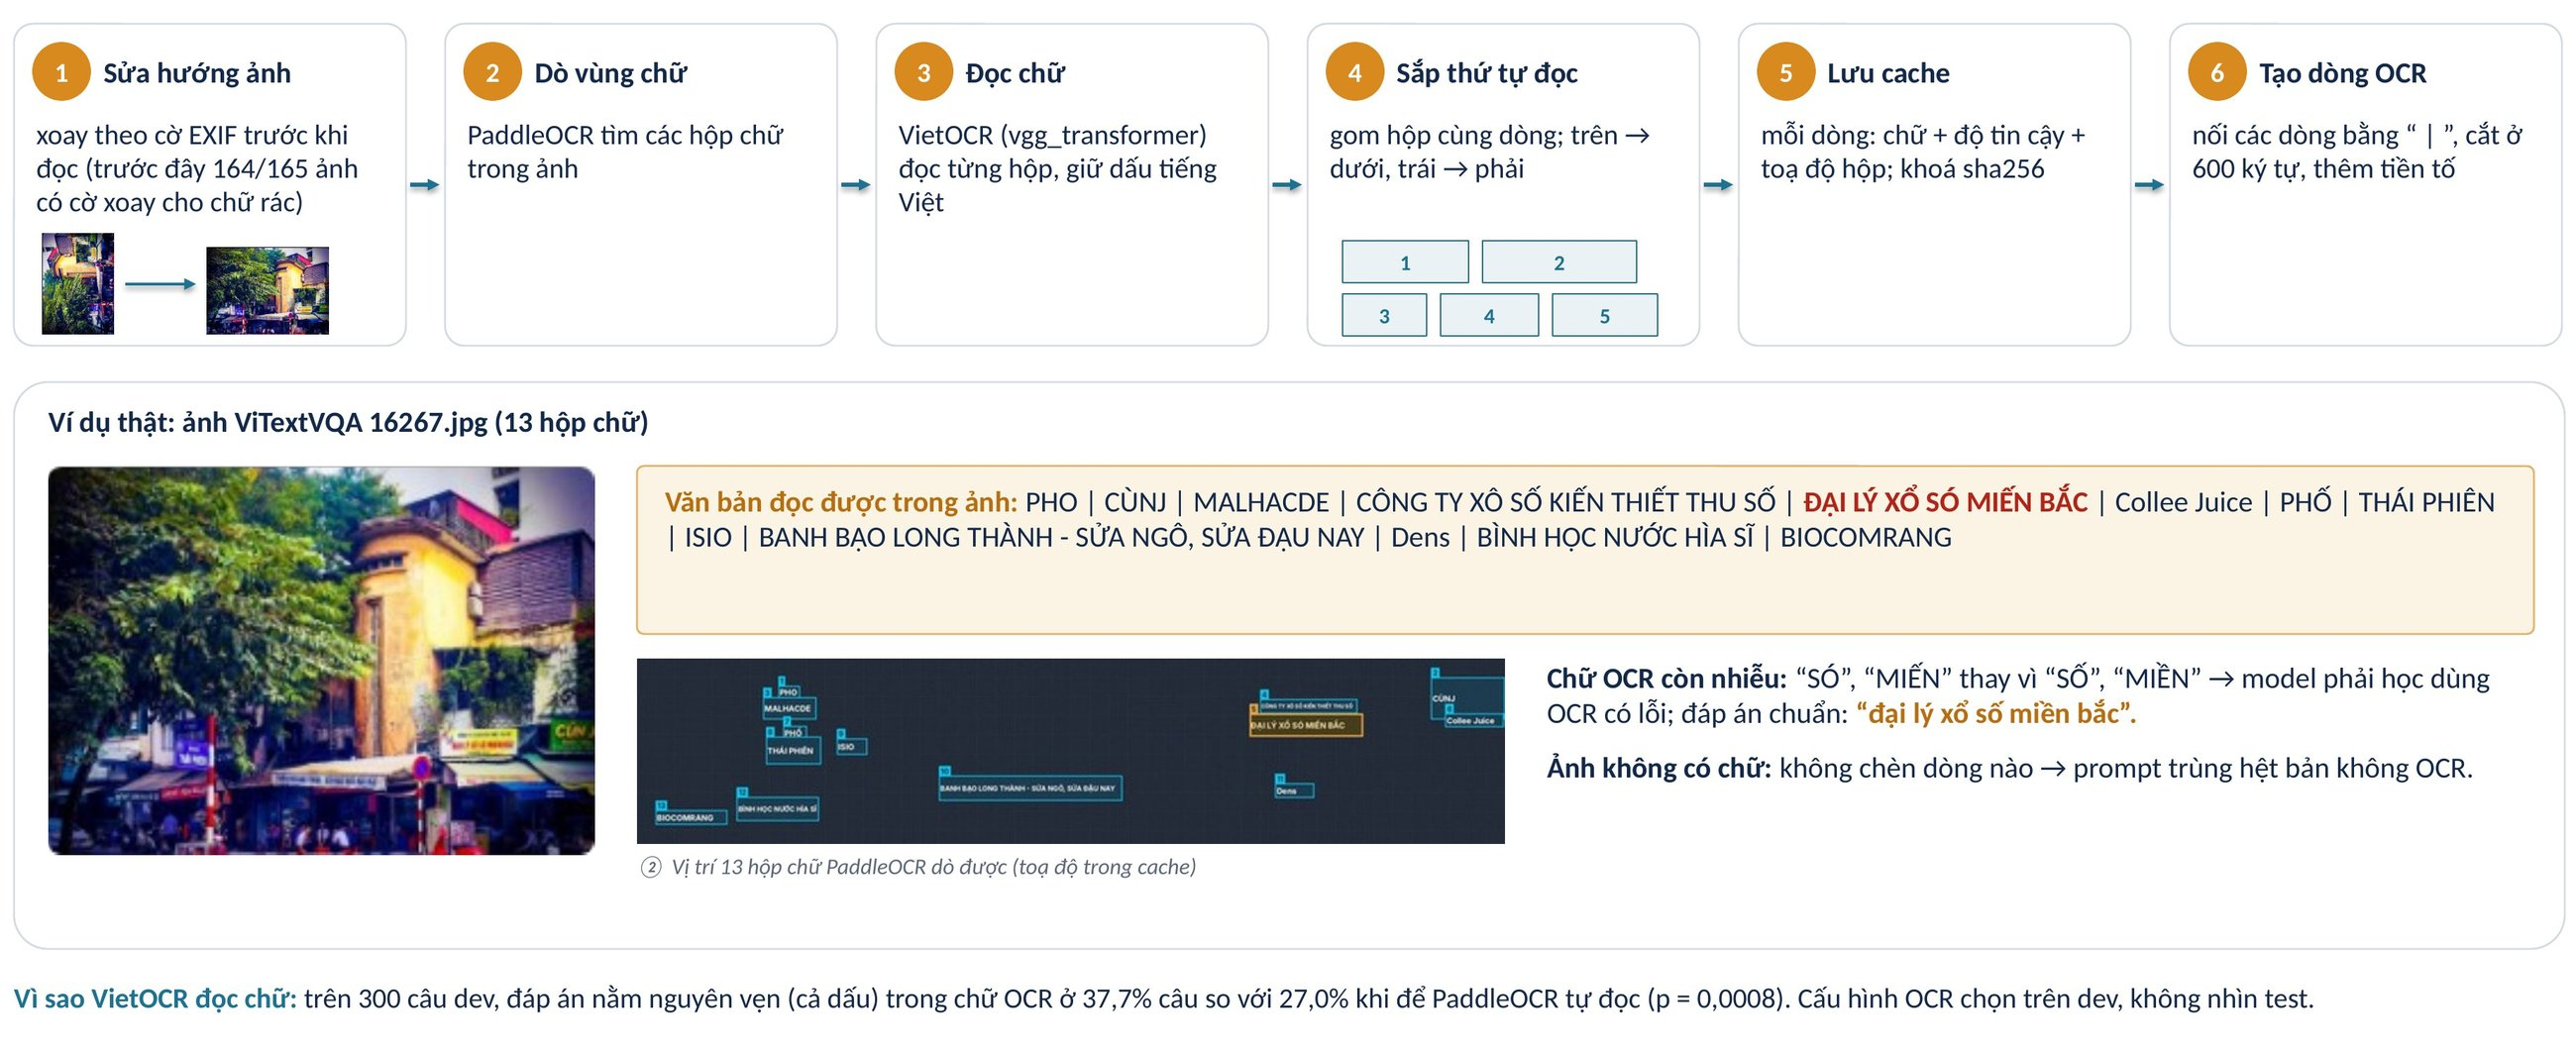
\includegraphics[width=\linewidth,height=0.82\textheight,keepaspectratio]{met_ocr.jpg}
\caption{Đường OCR trên ảnh ViTextVQA 16267.jpg: 13 hộp chữ được dò, đọc và nối thành
dòng OCR. Chữ OCR còn nhiễu (``SÓ'', ``MIẾN'' thay vì ``SỐ'', ``MIỀN''), trong khi đáp
án gold là ``đại lý xổ số miền bắc''.}
\label{fig:met-ocr}
\end{figure}
\end{landscape}

\subsection{Chọn cấu hình OCR}

Cấu hình OCR được chọn trên dev300 theo luật đặt trước, không nhìn tập test.
Tiêu chí chính là tỉ lệ câu có đáp án gold nằm nguyên văn, đúng cả dấu, trong chữ
OCR. PaddleOCR với mô hình đọc chữ Latin làm rơi dấu tiếng Việt (ví dụ ``Kiểu
Thẩm'' thành ``Kiu Thm''): đáp án nằm trong OCR ở 27,0\% câu nếu so giữ dấu,
nhưng 57,7\% nếu bỏ dấu khi so. Khi giữ bộ dò của PaddleOCR và thay phần đọc bằng
VietOCR, tỉ lệ so giữ dấu tăng lên 37,7\% (kiểm định McNemar $p = 0{,}0008$).
Nhóm chọn tổ hợp PaddleOCR dò và VietOCR đọc, mẫu tiền tố trung tính, cắt 600 ký
tự và không lọc theo độ tin cậy.

\subsection{Prompt}
\label{sec:met-prompt}

Phần chữ của prompt có hai dạng, khác nhau đúng một dòng:

\begin{itemize}
  \item Không OCR (B1, B2, C1, C3): ``Câu hỏi: \{câu hỏi\}''
  \item Có OCR (B3, B3-full, SH): ``Văn bản đọc được trong ảnh: \{dòng 1\}
  \textbar\ \{dòng 2\} \textbar\ \ldots'', xuống dòng, rồi
  ``Câu hỏi: \{câu hỏi\}''
\end{itemize}

Dòng OCR đặt trước câu hỏi để mô hình đọc nó như ngữ cảnh. Với một mẫu ViTextVQA
điển hình, chuỗi đầu vào gồm khoảng 62 token câu lệnh hệ thống và khuôn hội
thoại, 480 token ảnh, 76 token OCR và 11 token câu hỏi (giá trị trung vị trên
toàn tập). Chuỗi dài nhất trên toàn bộ dữ liệu là 1.058 token, chỉ bằng 0,83\%
cửa sổ ngữ cảnh 128.000 token của mô hình; giới hạn thực tế là VRAM và thời gian
huấn luyện, không phải độ dài ngữ cảnh.

\subsection{Huấn luyện B3 và B3-full}

B3 dùng đúng công thức của B2 (cùng siêu tham số, cùng 0,196\% tham số), chỉ thêm
dòng OCR vào prompt cả lúc huấn luyện lẫn lúc đánh giá. Nhóm kiểm chứng theo hai
bước. Bước một huấn luyện trên train8k và so với B2-sub, cùng tập con nhưng không
OCR; đây là phép thử có kiểm soát, rẻ và lặp lại được với nhiều seed. Bước hai
(B3-full) huấn luyện trên toàn bộ 35.159 câu train và so với B2 để trả lời câu
hỏi: khi đủ dữ liệu, OCR có còn giúp không.

%********************************** Mục 3.6 ************************************
\section{Giao thức đánh giá}
\label{sec:met-eval}

\subsection{Chuẩn hóa đáp án}
\label{sec:met-norm}

Trước khi so khớp, câu trả lời của mô hình và đáp án gold đi qua cùng một hàm
chuẩn hóa \texttt{normalize\_vi}, gồm sáu bậc cộng dồn:

\begin{description}
  \item[S1.] Unicode NFC: gộp chữ và dấu thành một mã thống nhất.
  \item[S2.] Chuyển chữ thường.
  \item[S3.] Bỏ dấu câu nhưng giữ dấu thanh tiếng Việt.
  \item[S4.] Gộp khoảng trắng thừa.
  \item[S5.] Bỏ tiền tố ``màu'' ở đầu chuỗi (``màu đỏ'' thành ``đỏ'').
  \item[S6.] Nếu cả chuỗi là một số (0--20 hoặc chục tròn đến 100), đổi chữ thành
  chữ số (``ba'' thành ``3'').
\end{description}

Hàm không bỏ dấu thanh (``con mèo'' khác ``con meo'') và không gộp từ đồng nghĩa,
nên EM giữ tính chặt chẽ; phần gần đúng do ANLS đo. Trên ViTextVQA, bậc S3 và S4
đổi 25,8\% đáp án gold (do gold viết tách dấu câu); trên ViVQA, bậc S5 và S6 đổi
20,9\% và 14,8\% đáp án. Mô hình đã huấn luyện gần như không phụ thuộc chuẩn hóa
(C3 đạt 76,6 ở mọi bậc), nên không bậc nào tự tạo ra cải tiến.

\subsection{Thước đo}

Gọi $p$ là câu trả lời và $G$ là tập đáp án gold, cả hai đã chuẩn hóa.

\paragraph{Exact Match (thước đo chính).} $\mathrm{EM}(p, G) = 1$ nếu $p$ trùng
khít một phần tử của $G$, ngược lại bằng 0.

\paragraph{VQA Accuracy.}
$\mathrm{Acc}(p, G) = \min\left(\#\{g \in G : g = p\}/3,\ 1\right)$ theo Antol và
cộng sự~\cite{antol2015vqa}. Trong cả hai bộ dữ liệu mỗi câu chỉ có một đáp án
gold, nên VQA-Acc trùng EM ở mọi lần chạy; khóa luận báo EM và ghi chú điều này.

\paragraph{ANLS.} Theo Biten và cộng sự~\cite{biten2019stvqa},
\begin{equation}
\mathrm{ANLS}(p, G) = \max_{g \in G} s(p, g), \qquad
s(p, g) =
\begin{cases}
1 - \dfrac{\mathrm{Lev}(p, g)}{\max(|p|, |g|)} & \text{nếu giá trị này } \geq 0{,}5,\\[6pt]
0 & \text{ngược lại,}
\end{cases}
\label{eq:anls}
\end{equation}
trong đó $\mathrm{Lev}$ là khoảng cách Levenshtein theo ký tự. ANLS chịu được lỗi
đọc nhỏ: ``miền bác'' so với ``miền bắc'' có EM bằng 0 nhưng ANLS bằng 0,95.

\paragraph{Token-F1 (chỉ số phụ).} F1 trên túi âm tiết của câu trả lời và gold,
chỉ dùng để so với số công bố của ViTextVQA. Vì khoảng trắng tiếng Việt tách âm
tiết chứ không tách từ, nhóm báo thêm F1 sau khi tách từ bằng pyvi để kiểm tra
kết luận không đổi.

BLEU và CIDEr không được dùng làm thước đo chính, đúng theo đề cương.

\subsection{Kiểm định thống kê}
\label{sec:met-stats}

Mọi so sánh giữa hai mô hình được thực hiện trên cùng một tập câu hỏi, nên nhóm
dùng kiểm định ghép cặp thay cho so sánh số tổng:

\begin{itemize}
  \item \textbf{EM}: kiểm định McNemar chính xác~\cite{mcnemar1947} (nhị thức
  hai phía) trên các câu chỉ một trong hai mô hình đúng.
  \item \textbf{ANLS, $\Delta$EM và hiệu ứng tương tác}: khoảng tin cậy 95\%
  bằng bootstrap ghép cặp~\cite{efron1993}, 10.000 lần lấy mẫu, seed 42.
  \item \textbf{Tỉ lệ trong duyệt tay}: khoảng tin cậy Wilson~\cite{wilson1927}.
  \item \textbf{POPE-vi}: bootstrap theo ảnh, vì các câu hỏi trên cùng một ảnh
  không độc lập.
\end{itemize}

Với 2.000 câu, ngưỡng $p < 0{,}05$ ứng với chênh lệch khoảng 1,7 điểm EM, và độ
mạnh kiểm định 80\% đạt khi chênh lệch thật khoảng 2,3 điểm. Các ablation trên
test2000 được đọc với giới hạn này.

\subsection{Luật quyết định ghi trước}

Trước mỗi thí nghiệm, nhóm ghi luật quyết định vào kho mã (commit có dấu thời
gian) rồi mới chạy. Luật nêu tập dữ liệu, mốc so sánh, thước đo, ngưỡng và cách
kết luận. Ví dụ: H1 được ủng hộ nếu QLoRA tăng EM ít nhất 5 điểm với $p < 0{,}05$;
adapter dùng chung được coi là ``không kém'' nếu cận dưới CI95 của $\Delta$EM lớn
hơn $-1{,}5$ trên từng bộ dữ liệu; một mô hình ``không tăng hallucination'' nếu cận
dưới CI95 của $\Delta$F1 trên POPE-vi lớn hơn $-2$. Khi kết quả không đạt luật,
nhóm báo đúng như vậy và không đổi luật sau khi đã thấy số.

\subsection{Đo hallucination: POPE-vi}
\label{sec:met-pope}

Nhóm xây POPE-vi, phiên bản tiếng Việt của POPE~\cite{li2023pope}. Ảnh là 500 ảnh
ViVQA test chưa từng xuất hiện trong train hoặc val; nhãn vật thể lấy từ chú
thích COCO 2014 và dịch sang tiếng Việt bằng một từ điển 80 lớp. Mỗi ảnh có ba
câu hỏi về vật có trong ảnh (đáp án ``có'') và ba câu hỏi về vật không có (đáp án
``không'') cho mỗi cách chọn vật vắng mặt: ngẫu nhiên (random), vật phổ biến
(popular) và vật hay đi kèm (adversarial). Mẫu câu dạng: Trong ảnh có \{vật\}
không? Trả lời ``có'' hoặc ``không''. Sau khi bỏ câu trùng còn 4.985 câu. Từ điển,
luật và file câu hỏi được khóa trong kho mã trước khi chạy mô hình.

Mỗi mô hình được so với chính mô hình nền zero-shot dùng cùng dạng prompt. Ngoài
F1 như cách báo cáo của LLaVA-1.5~\cite{liu2024llava15}, nhóm báo thêm tỉ lệ trả
lời ``có'' (yes-ratio), tỉ lệ báo sai (câu ``không'' bị trả lời ``có'') và tỉ lệ
câu trả lời không đọc được thành có hoặc không.

\subsection{Phân tích lỗi}
\label{sec:met-error}

Phân tích lỗi gồm hai phần. Phần tự động xếp mỗi câu sai EM vào một kiểu lỗi theo
thứ tự ưu tiên: chỉ khác dấu thanh, thiếu chữ, thừa chữ (gold nằm trong câu trả
lời), lệch không quá 2 ký tự, và còn lại. Với ViTextVQA, mỗi câu còn được xếp
theo trạng thái OCR: đáp án nằm nguyên văn trong OCR, chỉ khớp khi bỏ dấu, OCR có
chữ nhưng không chứa đáp án, hoặc OCR không đọc ra chữ. Định nghĩa được ghi trước
khi chạy. Phần duyệt tay lấy ngẫu nhiên (seed 42) 100 lỗi của B3-full và 50 lỗi
của C3, khóa danh sách trước khi gán nhãn, và gán nhãn mù: người gán chỉ thấy ảnh,
câu hỏi, gold và câu trả lời, không thấy kiểu lỗi tự động hay chữ OCR.

%********************************** Mục 3.7 ************************************
\section{Thiết lập thí nghiệm}
\label{sec:met-setup}

\paragraph{Phần cứng.} Mọi lần huấn luyện và đánh giá chạy trên một GPU NVIDIA L4
24~GB của Google Colab Pro. OCR chạy trên GPU Tesla T4 trong một phiên riêng.
Không lần chạy nào dùng quá một GPU.

\paragraph{Phần mềm.} Phiên bản thư viện được ghim trong
\path{requirements-colab.txt}: PyTorch 2.11.0, Transformers 5.17.0, PEFT 0.21.2,
bitsandbytes 0.50.2, Accelerate 1.15.0, qwen-vl-utils 0.0.14, PaddleOCR 3.x,
VietOCR và Gradio 6.31.0.

\paragraph{Log để tái lập.} Mỗi lần chạy ghi file chữ ký
\path{run_signature.json} (cấu hình và mã băm dữ liệu) cùng log kèm theo
(\path{train_log.json} khi huấn luyện; meta trong \path{metrics.json} khi đánh
giá), gồm split và mã băm file dữ liệu, seed, commit mã nguồn, loại GPU, phiên
bản thư viện, toàn bộ cấu hình, thời gian huấn luyện và suy luận, VRAM đỉnh.
Kết quả theo từng câu hỏi được lưu trong \path{predictions.json} để mọi thước đo
và kiểm định có thể tính lại từ đầu. Thư mục kết quả đặt tên ASCII theo quy ước
\begin{quote}\raggedright
\path|experiments/W<week>_<method>_<model>_<data>_<dtype>_<gpu>_seed<seed>/|
\end{quote}
(có thể xen thêm token phụ như hạng LoRA hay số epoch). Trong đó \texttt{week}
là tuần thí nghiệm, \texttt{method} là phương pháp, \texttt{model} là mô hình,
\texttt{data} là tập dữ liệu, \texttt{dtype} là kiểu số, \texttt{gpu} là GPU và
\texttt{seed} là hạt giống ngẫu nhiên. Ví dụ thư mục có thật:
\begin{quote}\raggedright
\path{experiments/W07_B2_qlora_r16_qwen25vl_vitextvqa_ep1_bf16_L4_seed42/}
\end{quote}

%********************************** Mục 3.8 ************************************
\section{Thiết kế prototype}
\label{sec:met-proto}

Prototype là một ứng dụng web Gradio~\cite{abid2019gradio} chạy trên Colab L4.
Người dùng tải ảnh lên và đặt câu hỏi tiếng Việt; hệ thống trả lời kèm chữ OCR và
mức tin cậy. Thiết kế tuân theo ba nguyên tắc:

\begin{enumerate}
  \item \textbf{Cùng một đường suy luận với đánh giá.} Prototype gọi đúng hàm dựng
  prompt, đúng adapter và đúng cách sinh câu trả lời (greedy, tối đa 32 token)
  của đường đánh giá. Điều này được kiểm bằng luật trùng khớp ở
  mục~\ref{sec:res-proto}.
  \item \textbf{Câu trả lời kèm bằng chứng.} Vì mô hình dùng OCR, giao diện hiển
  thị chữ OCR đọc được để người dùng tự kiểm tra câu trả lời. OCR chạy trong một
  tiến trình riêng, đọc ảnh gốc (tối đa 6.000 điểm ảnh mỗi cạnh) đã xoay theo cờ
  EXIF.
  \item \textbf{Một adapter cho mọi câu hỏi.} Prototype dùng adapter SH, huấn
  luyện trên cả ViVQA và ViTextVQA, để không phải đoán trước người dùng hỏi loại
  câu nào.
\end{enumerate}

\paragraph{Độ tin cậy.} Với câu hỏi mở, độ tin cậy là $\exp$ của trung bình log
xác suất các token trả lời. Vì độ tin cậy này chưa được hiệu chỉnh tốt
(ECE~\cite{guo2017calibration} bằng 0,198), giao diện chỉ hiện mức Cao, Trung bình
hoặc Thấp thay cho con số phần trăm.

\paragraph{Câu hỏi có/không.} Một bộ nhận diện theo luật đánh dấu câu hỏi có/không
(kết thúc bằng ``không'', ``chưa'', ``phải không''\ldots và không chứa từ để hỏi).
Với các câu này, quyết định dựa trên hiệu $m = s_{\text{có}} - s_{\text{không}}$
giữa log xác suất lớn nhất của token đầu phía ``có'' và phía ``không'': trả lời
``có'' khi $m > \tau^*$. Ngưỡng $\tau^* = 4{,}85$ được chọn trên một tập hiệu
chỉnh riêng (ảnh ViVQA test chưa thấy khi huấn luyện, không thuộc POPE-vi) bằng
cách tối đa balanced accuracy, để sửa thiên lệch ``có'' của SH
(mục~\ref{sec:dis-halluc}) mà không phải huấn luyện lại. Câu hỏi khác vẫn đi
đường greedy như khi đánh giá.

\paragraph{Quyền riêng tư.} Prototype không lưu ảnh hay câu hỏi của người dùng;
chỉ ghi thời gian xử lý.
